\begin{surferPage}[Површ са 15 шиљака]{Површ петог реда са 15 шиљака}
  Површ петог степена има 15 сингуларитета типа $A_2$
    (званих шиљак). Ова површ и низ сличних површи су представљене у  раду Оливера 
	Лабса из 2005. године.
    Пет шиљака се разликује по изгледу од осталих 10.
    Наиме, пет је типа $A_2^{++}$ а остале су типа $A_2^{+-}$ (погледајте галерију 
	простих сингуларитета за више информација):

     \vspace*{-0.3em}
    \begin{center}
      \begin{tabular}{c@{\qquad}c}
        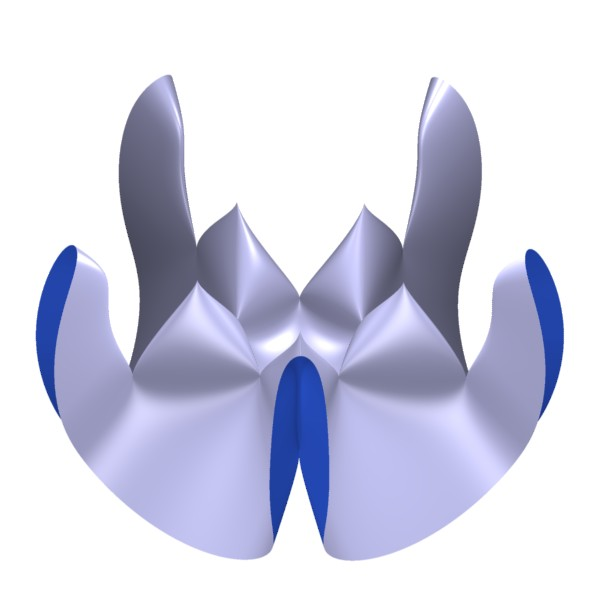
\includegraphics[height=1.2cm]{./../../common/images/dessins_quint_15a2}
        &
        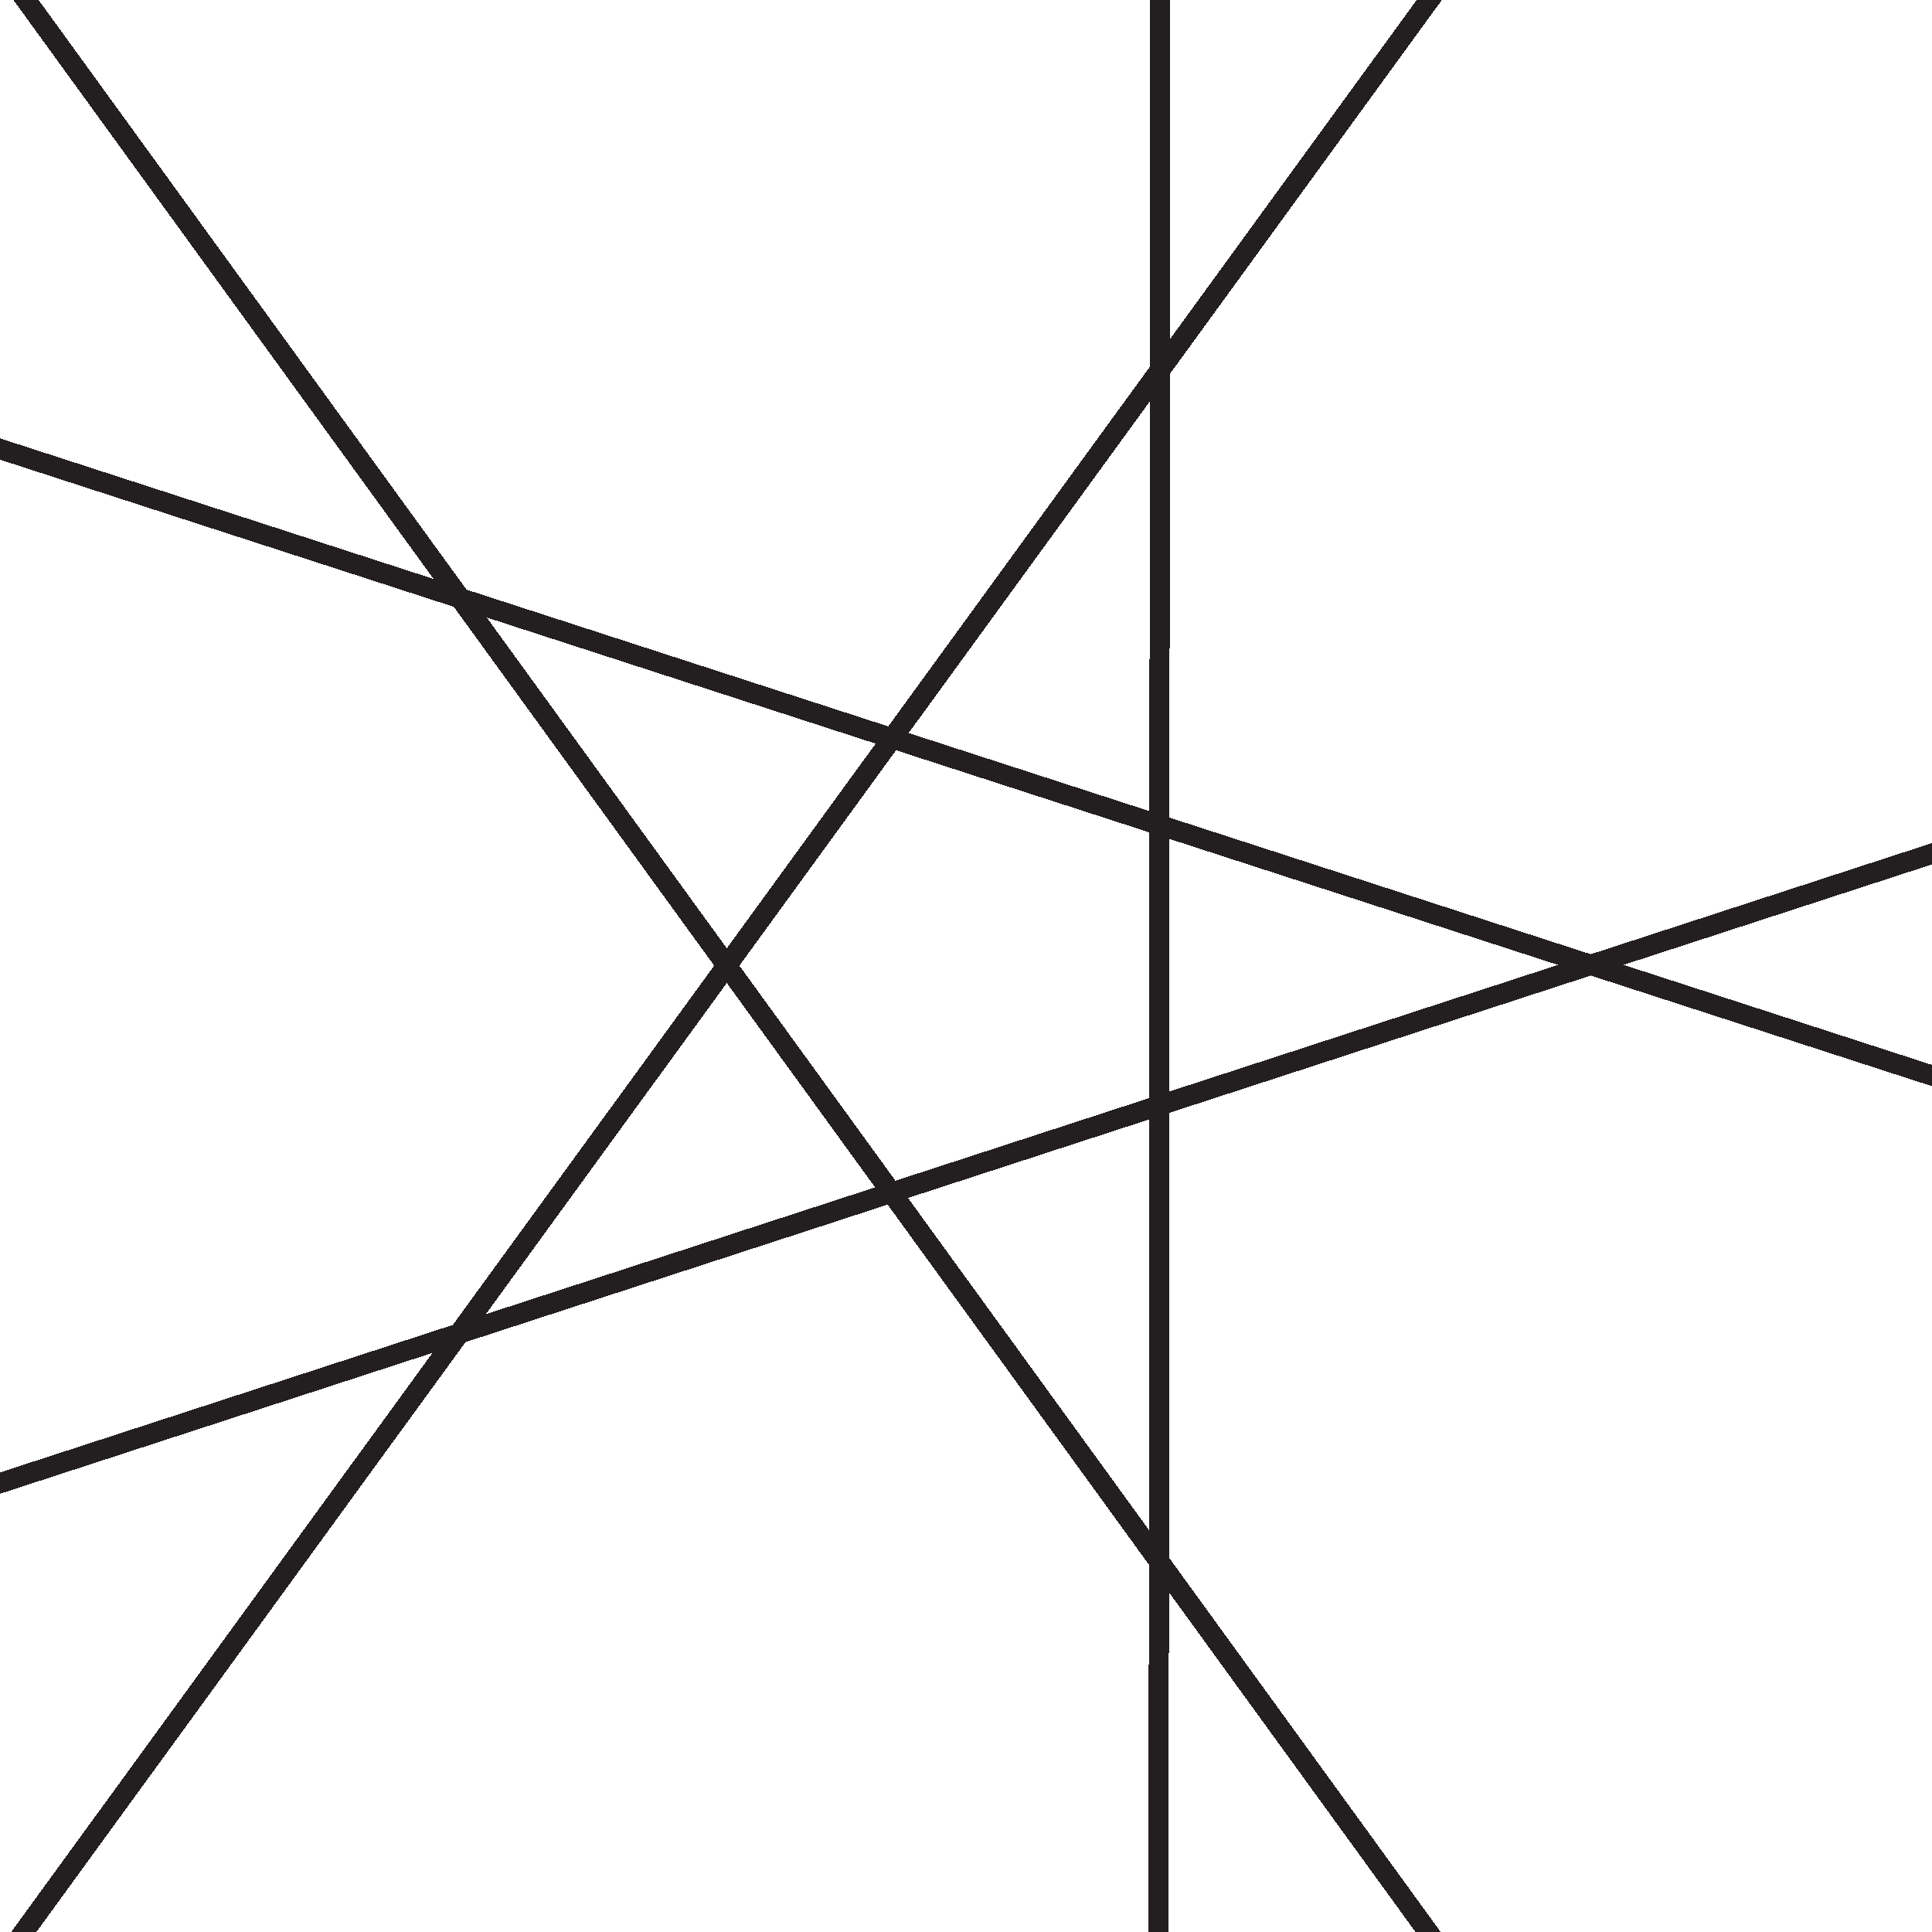
\includegraphics[height=1.2cm]{./../../common/images/rp5.pdf}
      \end{tabular}
    \end{center}
    \vspace*{-0.3em}    
    
    Ова површ има једначину  
    $S_5(x,y) + t(z)=0,$
    где је $S_5(x,y)$ правилни петоугао (слика десно) и $t(z)$ је варијанта 
	Чебишевљевих полинома коју смо већ неколико пута помињали.

     Још једну површ петог реда са 15 шиљака је конструисао Волф Барт; 
	 повезана је са Клебшовом површи трећег реда (десно) што се може видети на средњој слици:

    \vspace*{-0.3em}
    \begin{center}
      \begin{tabular}{c@{\quad}c@{\quad}c}
        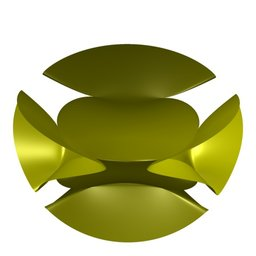
\includegraphics[height=1.2cm]{./../../common/images/barthquintic_green}
        &
        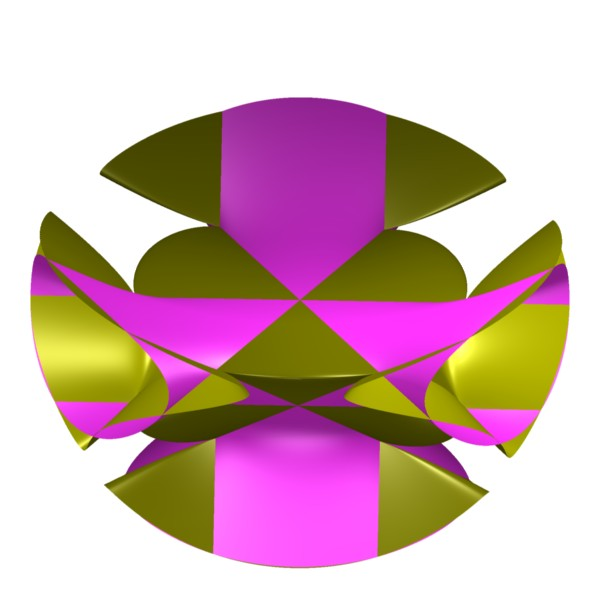
\includegraphics[height=1.2cm]{./../../common/images/barthquintic_clebschcubic}
        &
        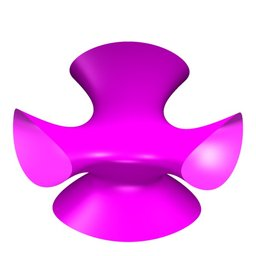
\includegraphics[height=1.2cm]{./../../common/images/clebschcubic_pink}
      \end{tabular}
    \end{center}
    \vspace*{-0.3em}
\end{surferPage}
